\documentclass[12pt]{article}

\usepackage{amsmath,amssymb,amsthm}
\usepackage{graphicx}
\usepackage[margin=1in]{geometry}

\begin{document}


\section{Application of Hedging for Historical Positions in Uniswap Pool ETH/USDT}
\label{sec:hedgingmechanism}

We propose an initial hedging methodology by leveraging Uniswap V4's latest hook capabilities to open hedging perpetual positions with mirror funds on the GMX exchange. The goal is to mitigate impermanent loss by stabilizing the payoff function to be market neutral and, when possible, improve market efficiency for Uniswap while enhancing collected fees for the user. The hook mechanism automates the process of splitting initial funding, ensuring seamless integration of the hedging strategy within Uniswap’s smart contract framework.

\subsection{Hedging Mechanism}

\paragraph{Liquidity Provision Setup:} 
We presume entering hedged lp position is the same as in Uniswap v3.
\begin{itemize}
    \item $P_L$: The lower bound price of the LP position (USDT per ETH).
    \item $P_U$: The upper bound price of the LP position (USDT per ETH).
    \item $X_0$: The amount of ETH (token0) held at the time the position is set, related to $P_U$ and $P_L$.
    \item $Y_0$: The amount of USDT (token1) held at the time the position is set, also related to $P_U$ and $P_L$.
\end{itemize}
The total value of deposited tokens is considered the user's original investment.

\paragraph{Triggering the Hedging Mechanism:} 
The hedging mechanism is activated only when Xtreamly AI predicts 'low volatility.' This ensures that hedging is only applied in stable market conditions, reducing the risk of perpetual liquidation due to sudden price swings.

\paragraph{Fund Allocation at Position Opening:} 
We presume entering hedged lp position is the same as in Uniswap v3.
\begin{itemize}
	\item \textbf{80\%} of the funds are allocated to the Uniswap LP position, structured with the same price bounds as the original deposit but proportionally reduced.
	\item \textbf{20\%} is allocated to a hedging perpetual futures position.
\end{itemize}

\paragraph{Perpetual Hedge Positioning:} 

\begin{itemize}
	\item The perpetual hedge is a short position using the allocated 20\% as collateral.
	\item The leverage is determined to ensure that the liquidation price of the perpetual position is slightly above the upper price bound, using the formula:
	$$Leverage_GMX = int(\min(10,\max(1,  \frac{1}{\frac{P_U}{P}-1})))$$
	where $\max 10$ relates to 10\% of the price buffer; and $\min 1$ avoid excessively loose hedging ranges.
\end{itemize}
This approach accounts for the highly volatile nature of Uniswap pools and optimizes the risk-reward balance in the hedging strategy. 

\subsection{Assumptions on GMX Parameters}
The following GMX trading parameters are assumed:
\begin{itemize}
	\item \textbf{Entry fee}: 0.1\%
	\item \textbf{Exit fee}: 0.1\%
	\item \textbf{Gas fee}: Considered negligible due to GMX's efficient execution model.
	\item \textbf{Funding rate}: 0.01\% (assumed constant and charged on an hourly basis).
	\item \textbf{Maximum perpetual duration}: 24 hours. Due to the perpetual funding rate cost, positions cannot be held indefinitely without eroding hedging benefits.	
\end{itemize}

\subsection{Assumptions on Selecting Uniswap Positions for Backtesting}
For backtesting, we identified LP Positions in Uniswap Pool ETH/USDT 0.3\% Fee, that will be used to evaluate the effectiveness of our hedging strategy under different market conditions, comparing LP-only positions against LP positions with perpetual hedging.

\paragraph{Selection Criteria:}
To ensure computational simplicity and practical relevance, we apply the following selection constraints:
\begin{itemize}
	\item \textbf{Period}: LP positions must have been opened and closed between 2024-10-01 and 2024-12-31.
	\item \textbf{Minimum duration}: 60 minutes to avoid Just-In-Time (JIT) positions and ensure sufficient market impact assessment.
	\item \textbf{Concentration levels}: The difference between upper and lower price bounds relative to the deposited price must not exceed 30\%. This aligns with Uniswap V3 \& V4 efficient liquidity allocation principles, ensuring that leveraged hedging is effective.
	\item \textbf{Simplistic positions}: We select only positions consisting of three transaction logs: deposit tokens, withdraw tokens, and collected fees. This simplification facilitates efficient backtesting as a tradeoff of simplicity.
	\item \textbf{No assumptions on position value}: The strategy is applied across a range of liquidity sizes.
\end{itemize}
By applying these filters, we ensure realistic hedging conditions where the strategy remains both practical and effective.

\subsection{Monitoring Performance of Hedged LP Positions}
To evaluate performance, we simulate LP positions and perpetual positions simultaneously by applying the hedging mechanism to historical data.

\paragraph{Sample Position Hedging}
Given the criteria and mechanism described before, here is a sample hedging visualization of position ID \textbf{$840439_0x4942e2b839fc479c27c496b7758bab94ceb6b684$}.
\begin{figure}[htb]
	\centering
	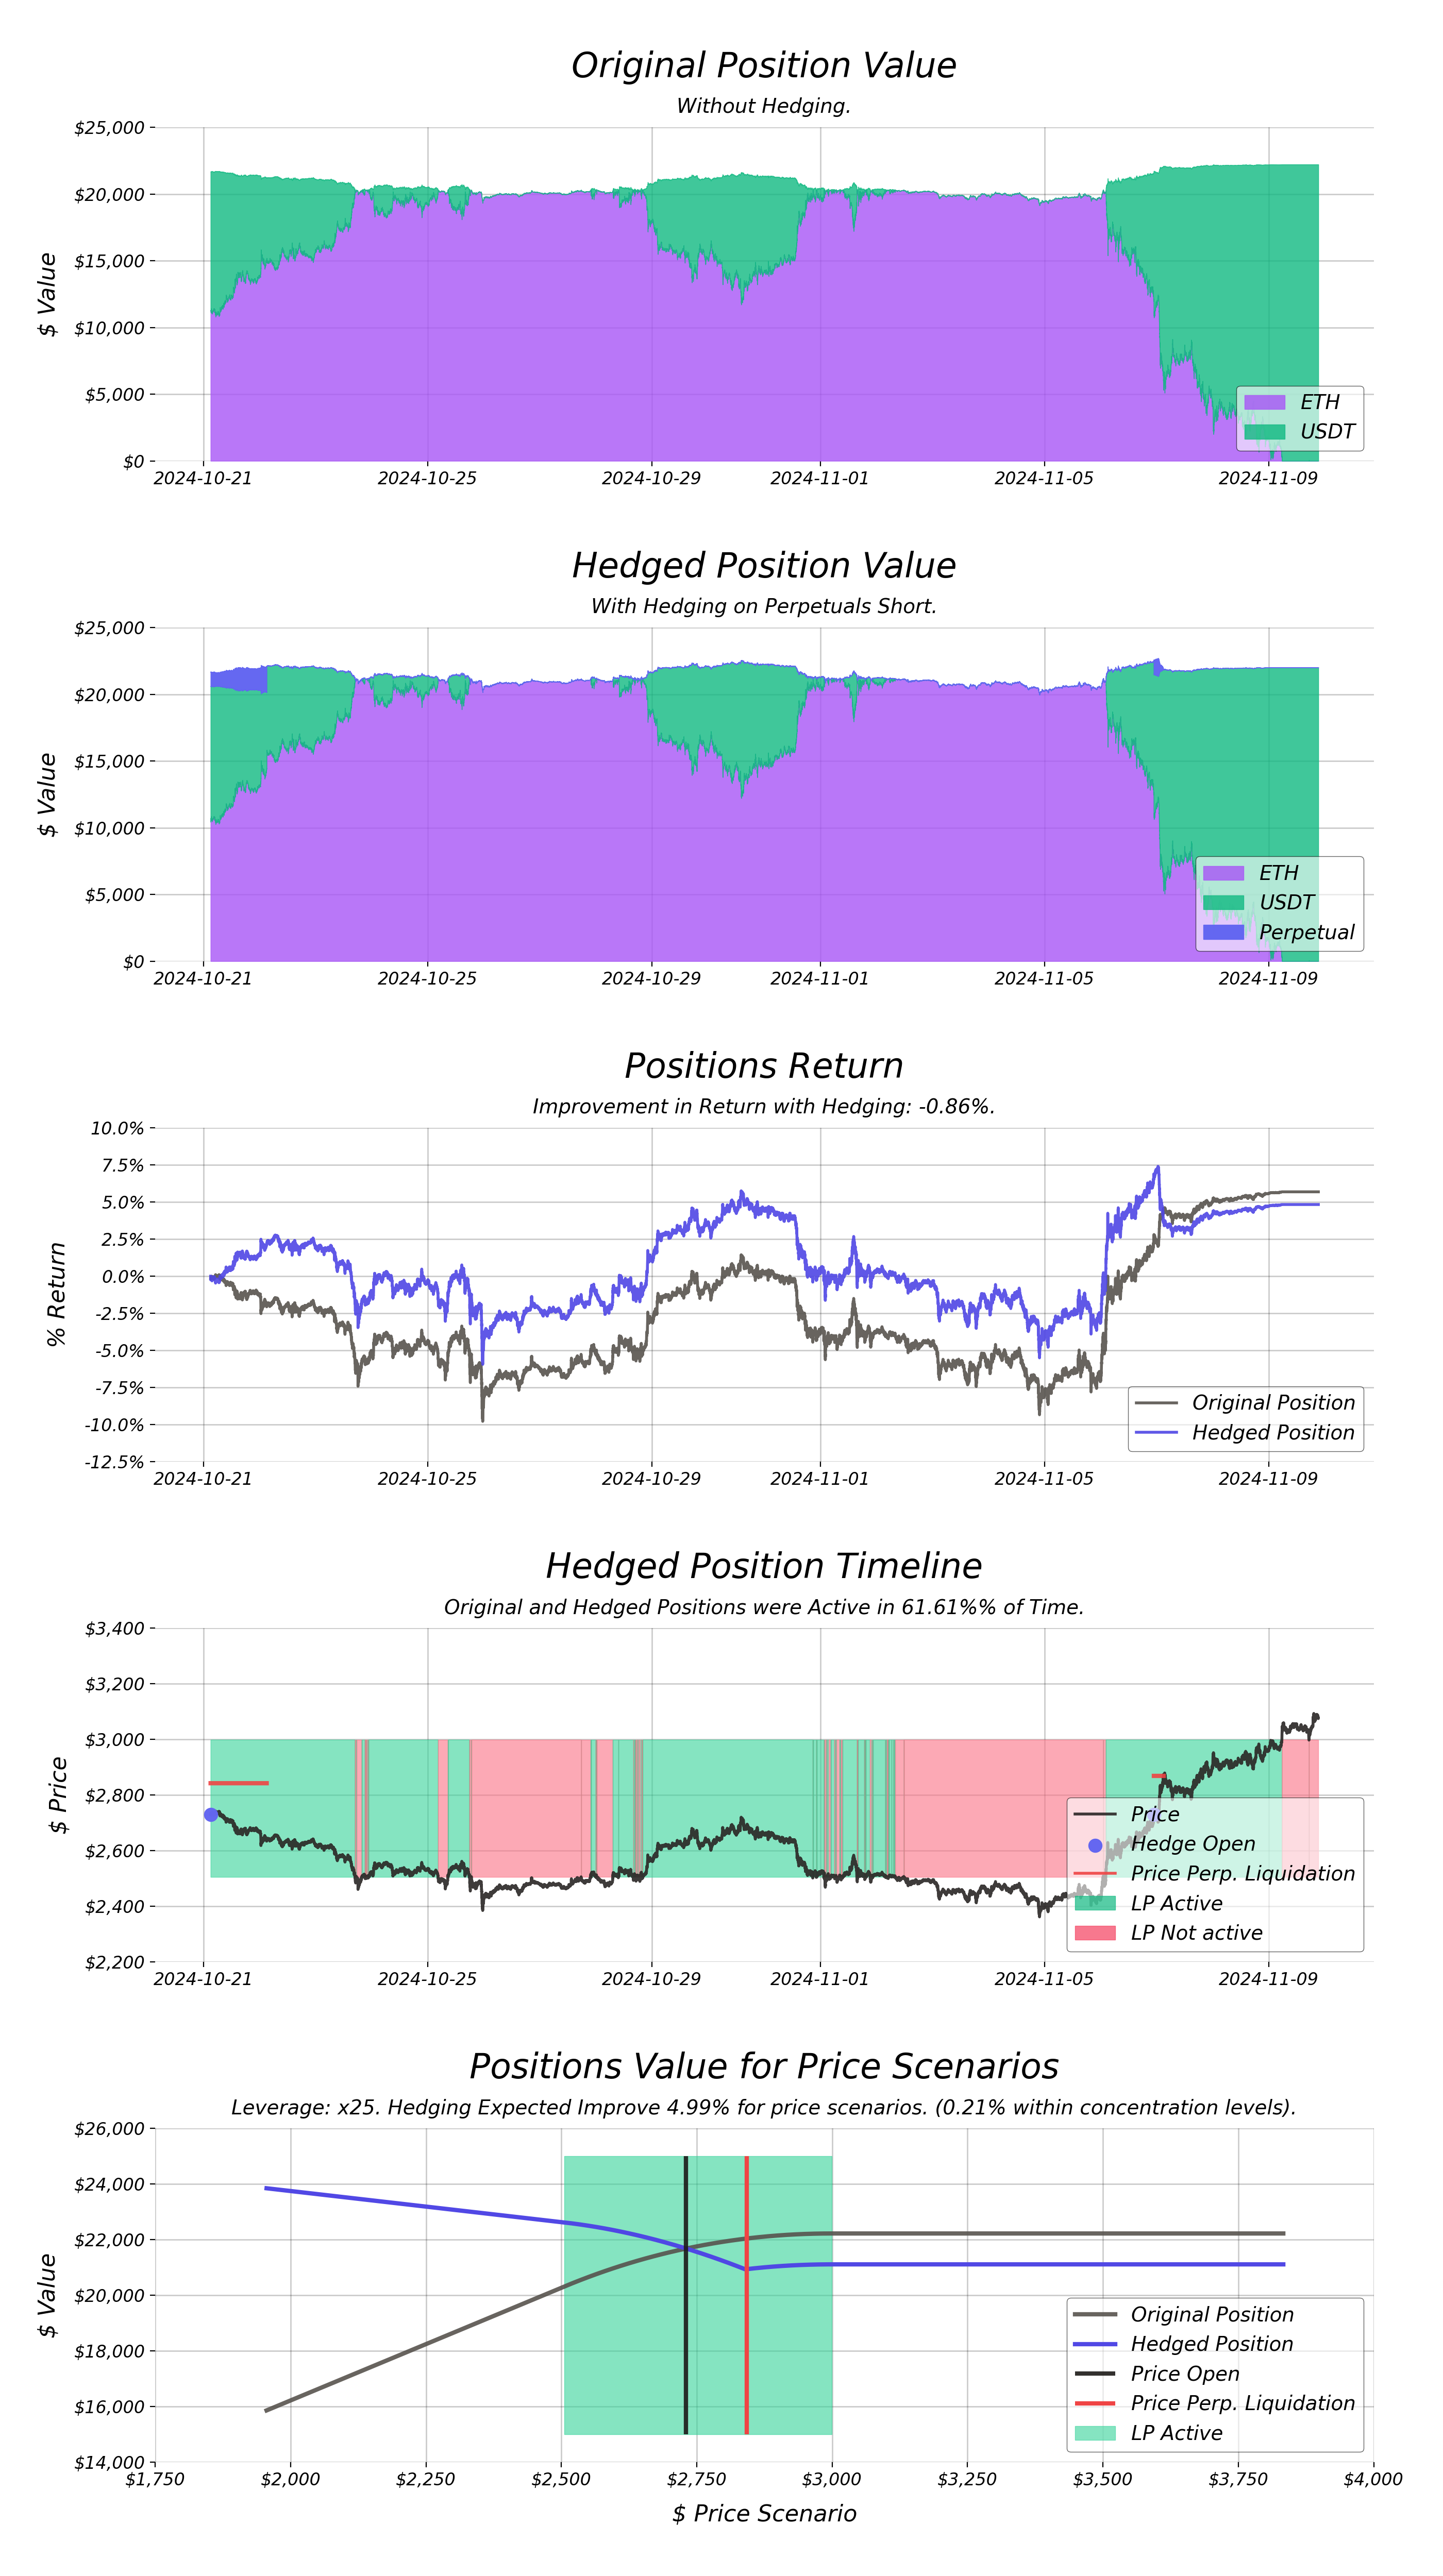
\includegraphics[width=0.7\textwidth]{images/Position Hedge 840439_0x4942e2b839fc479c27c496b7758bab94ceb6b684.png}
	\caption{illustrating the hedged V4 position timeline.}
	\label{fig:Sample}
\end{figure}

\paragraph{Aggregated Position Hedging}
For aggregated positions, we have applied extra differentiation based on market status predicted by Xtreamly AI.

\begin{table}[htb]
	\centering
	\includegraphics[width=0.99\textwidth]{images/Aggr table.png}
	\caption{illustrating the aggregated improvement for hedged V4 position depending on market status at position open.}
	\label{fig:Agr}
\end{table}

\begin{figure}[htb]
	\centering
	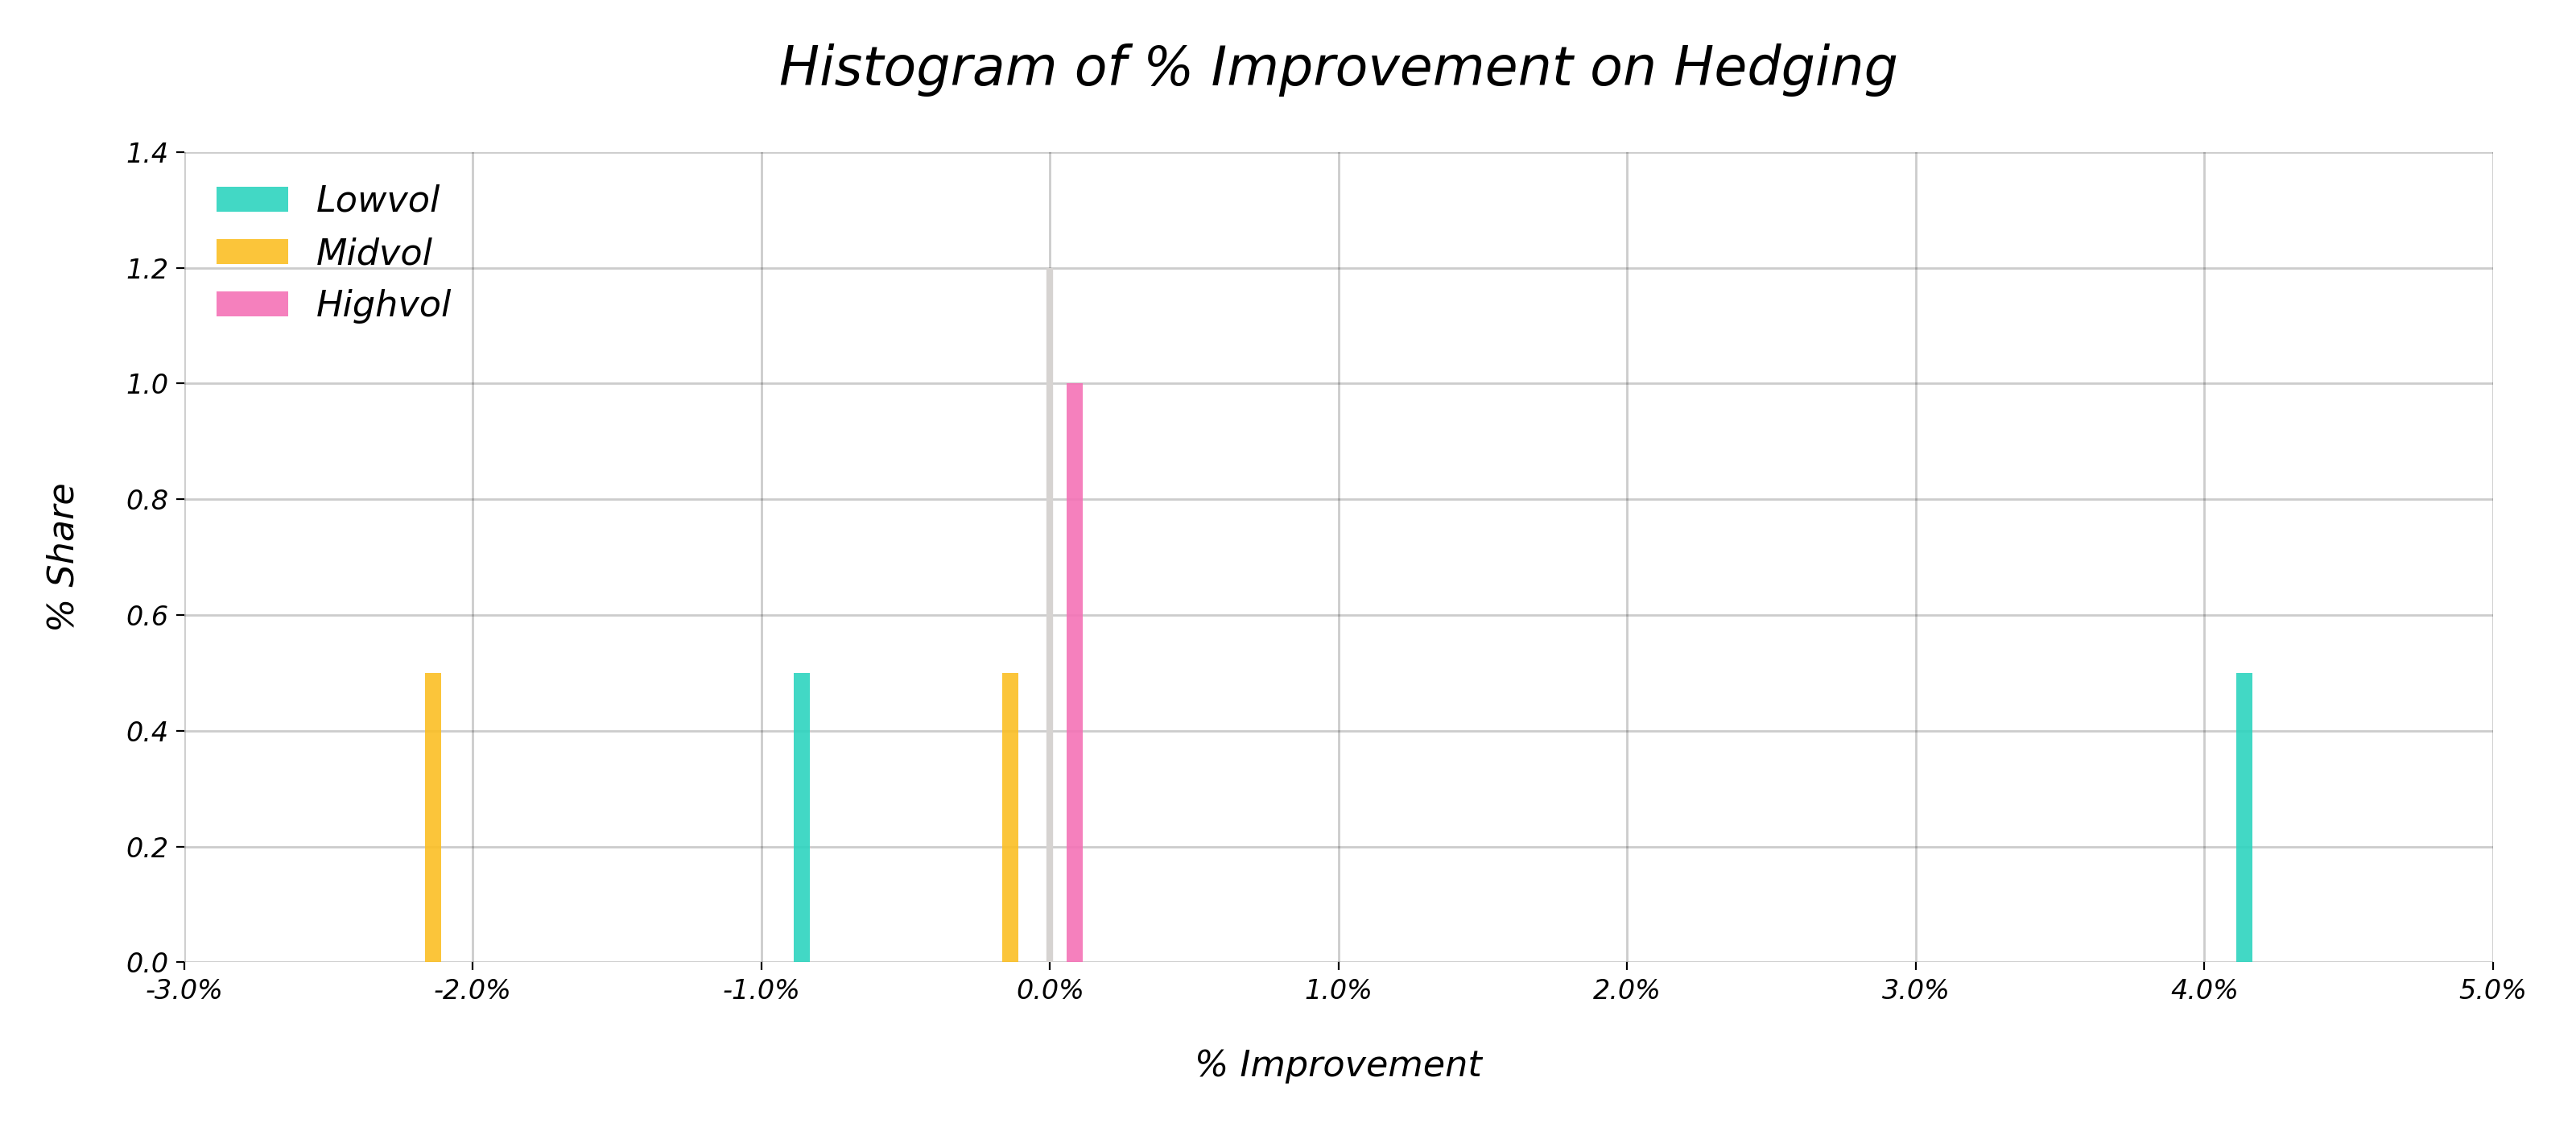
\includegraphics[width=0.8\textwidth]{images/Histogram Improvement.png}
	\caption{illustrating the improvement distribution depending on market status at position open.}
	\label{fig:HistImprov}
\end{figure}

We observe clear added value for positions opened during low volatility periods. This is partly due to the reduced perpetual liquidations as well as the skewness of the payoff function, favoring perpetuals as an implementation of a market-neutral position whenever the market regime is in low volatility.

\newpage

\section{Further Work}
\label{sec:futurework}

\subsection{Further and Deeper Analysis}
Expand analysis to other pools and tokens, seeking data signals for opening perpetual hedging.

\subsection{Intelligent Hedging Momentum}
Use Xtreamly AI volatility predictions to more intelligently define opening and closing of perpetuals.

\subsection{Reinvesting Closed Perpetual into ne LP position}
Reuse PnL and collateral from closed perpetual exposure to create new LP positions, so the liquidity can be reapplied back to Uniswap and user can collect more fees.

\subsection{Automated Rebalancing and Hedging Investment Vechicle}
Develop automated rules for managing hedging exposure and rebalancing LP positions.

\subsection{New Hedging Intruments}
Explore Panoptic platform for DeFi options trading to secure hedging during high volatility periods.

\newpage

\section{Reference}
\label{sec:ref}
To fill in.
\begin{itemize}
	\item \textbf{Uniswap Documentation}
	\item \textbf{GMX Documentation}
	\item \textbf{Other}
\end{itemize}



\end{document}